\section{Aufbau des Versuchs}
%Bild vom Aufbau einfügen, entweder Online/in Litteratur finden oder eigenes Foto machen
\begin{figure}[htbp]
    \centering
    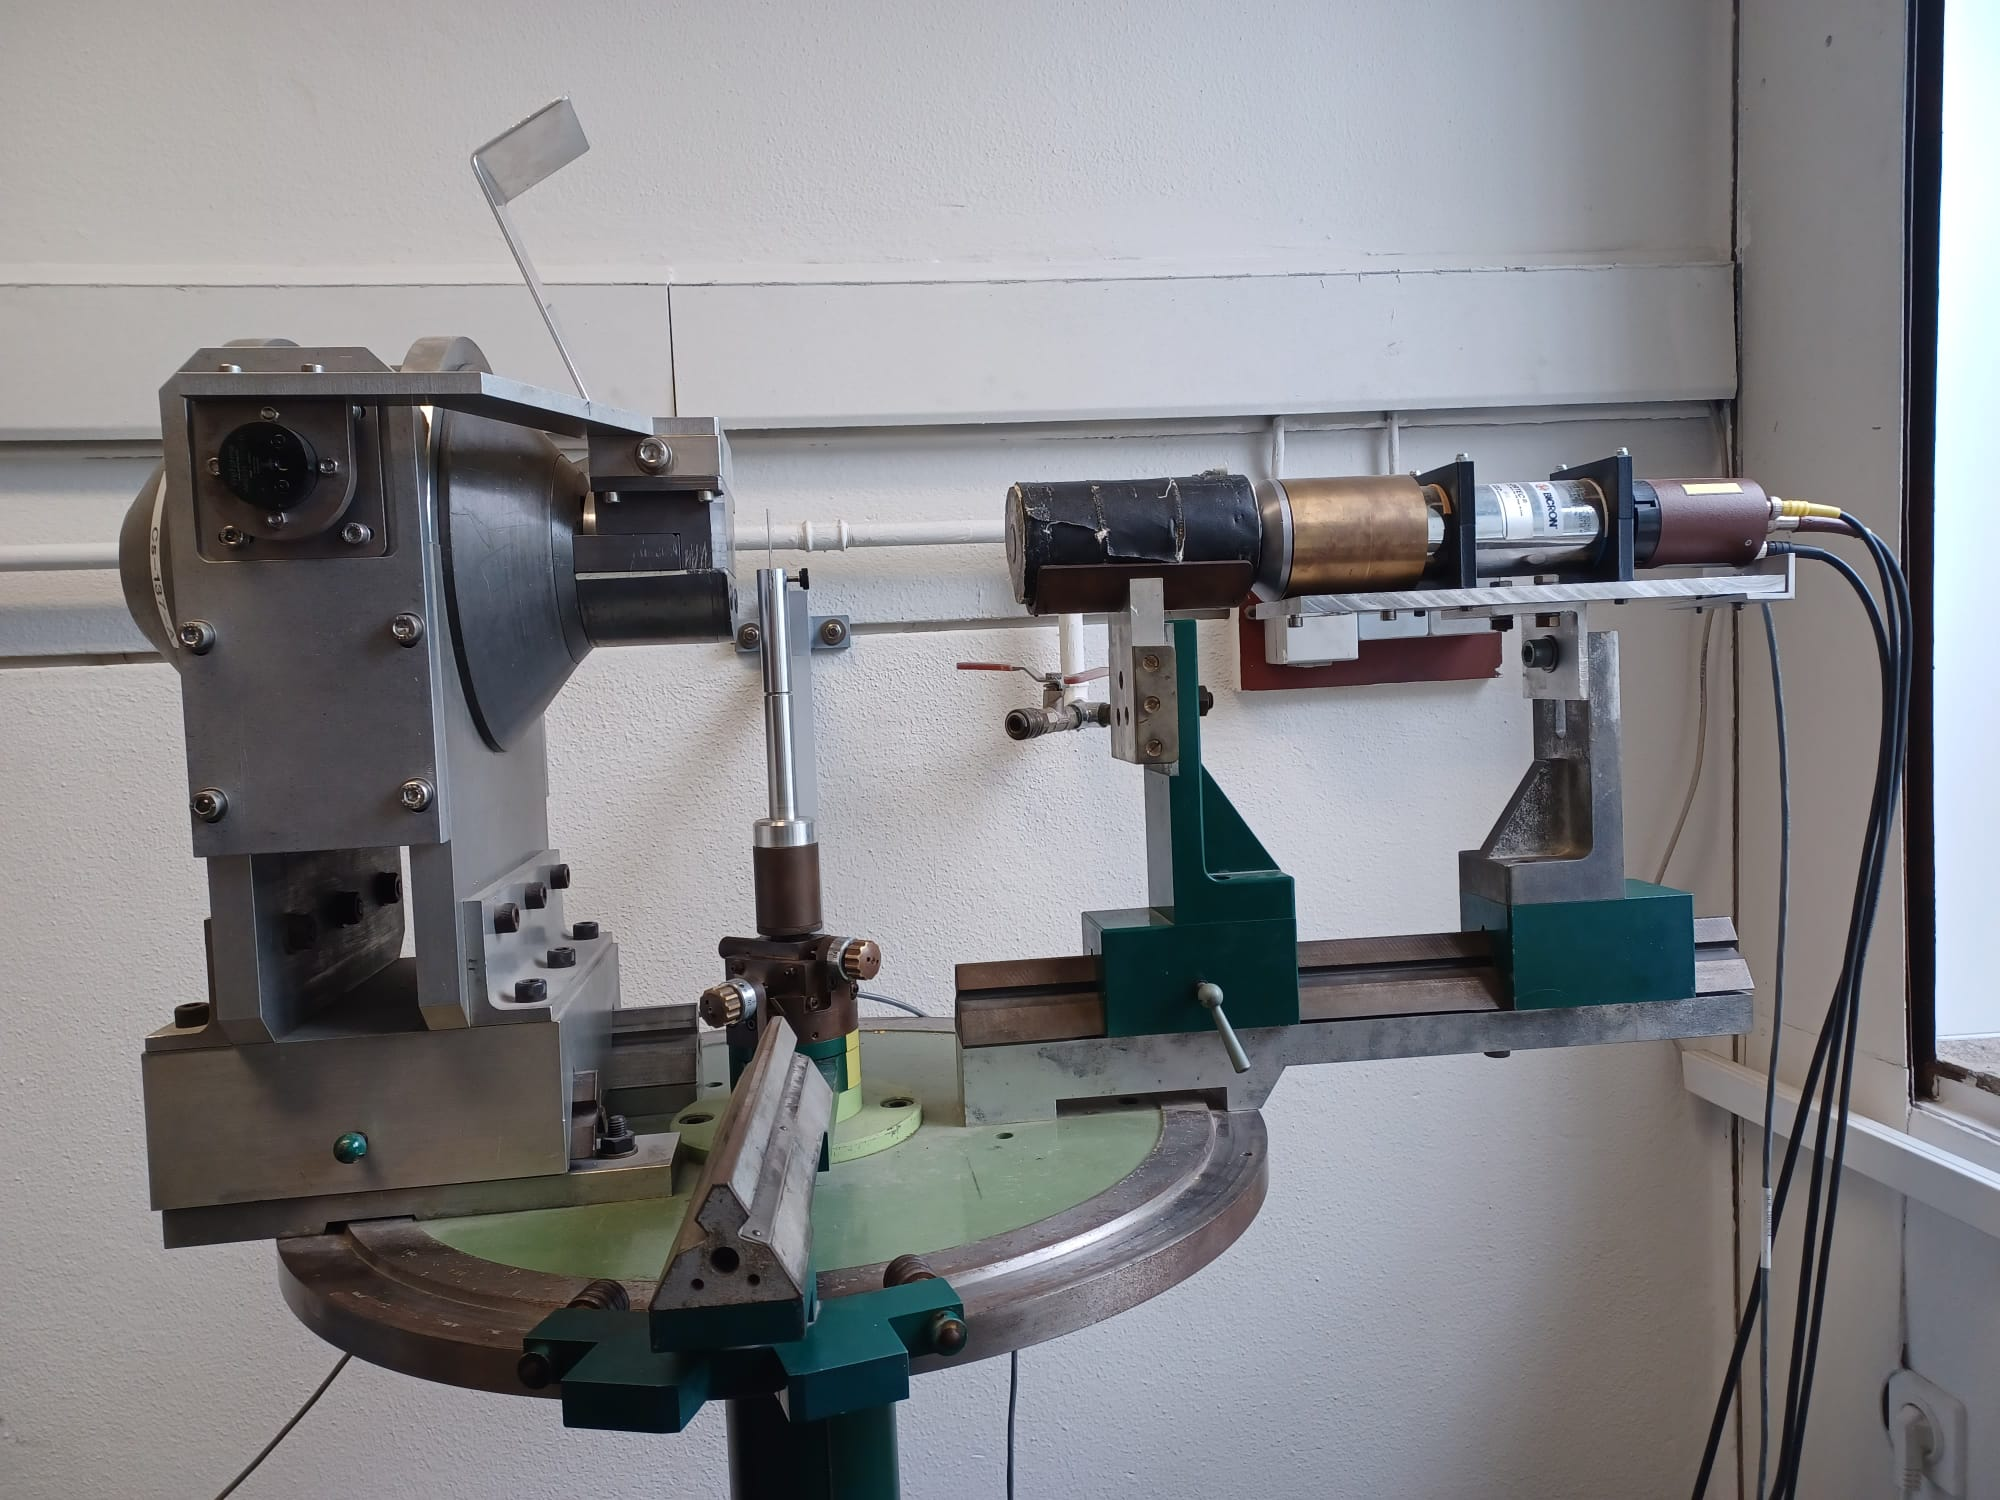
\includegraphics[width=0.75\textwidth]{figs/photo_aufbau.jpeg}
    \caption{Versuchsandornung für die Messungen der Compton-Streuung und der Energiekalibrierung.}
    \label{fig:aufbau1}
\end{figure}
\FloatBarrier
Die obbige Abbildung (\ref{fig:aufbau1}) veranschaulicht den für die Messungen verwendeten Strahlengang. Am linken Ende befindet sich die $^{137}\text{Cs}$-Probe in einem abgeschirmten, mechanisch geschlossenen Probenhalter, der eine kontrollierte Emission von $\kappa$-Strahlung ermöglicht. Unmittelbar rechts davon befindet sich der Targethalter, der ein Aluminiumtarget für Compton-Streuungsuntersuchungen oder eine $^{152}\text{Eu}$-Probe zur Energiekalibrierung des Szintillationsspektrometers aufnehmen kann.

Weiter entlang des Strahlengangs befindet sich ein Kollimator mit 1 mm Durchmesser, der die Dispersion der einfallenden $\kappa$-Strahlung reduziert und somit eine definierte Geometrie für die Wechselwirkung mit dem Target gewährleistet. Dahinter, in Messrichtung, befindet sich das Szintillationsspektrometer, dem ein zweiter Kollimator mit 3 cm Durchmesser vorgeschaltet ist. Diese beiden Elemente sind beweglich und können auf der zweiten Messschiene positioniert werden, um die Streuspektren in Abhängigkeit vom Winkel aufzuzeichnen. Das vom Szintillator erzeugte analoge Signal wird anschließend an einen externen Messverstärker übertragen und digitalisiert.

%Bild mit aufbau für den 2. Versuchsteil

Wenn das Szintillationsspektrometer, wie in Abbildung (\ref{fig:aufbau}) dargestellt, an Position im direkten Strahlengang positioniert ist, wird diese Konfiguration als Konfiguration 1 bezeichnet. Wenn das Spektrometer jedoch auf der zweiten Messschiene positioniert ist, um gestreute Photonen zu erfassen, entspricht dies der Konfiguration 2.